\documentclass{beamer}
\usetheme{Madrid}

\usepackage{listings}

\AtBeginSection[]{
  \begin{frame}
  \vfill
  \centering
  \begin{beamercolorbox}[sep=8pt,center,shadow=true,rounded=true]{title}
    \usebeamerfont{title}\insertsectionhead\par%
  \end{beamercolorbox}
  \vfill
  \end{frame}
}

\makeatletter
\setbeamertemplate{footline}{%
  \leavevmode%
  \hbox{%
  \begin{beamercolorbox}[wd=.2\paperwidth,ht=2.25ex,dp=1ex,center]{author in head/foot}%
    \usebeamerfont{author in head/foot}\insertshortauthor\expandafter\beamer@ifempty\expandafter{\beamer@shortinstitute}{}{~~(\insertshortinstitute)}
  \end{beamercolorbox}%
  \begin{beamercolorbox}[wd=.4\paperwidth,ht=2.25ex,dp=1ex,center]{title in head/foot}%
    \usebeamerfont{title in head/foot}\insertshorttitle
  \end{beamercolorbox}%
  \begin{beamercolorbox}[wd=.4\paperwidth,ht=2.25ex,dp=1ex,right]{date in head/foot}%
    \usebeamerfont{date in head/foot}\insertshortdate{}\hspace*{2em}
    \insertframenumber{} / \inserttotalframenumber\hspace*{2ex} 
  \end{beamercolorbox}}%
  \vskip0pt%
}
\makeatother


%Packages
\usepackage{xcolor}
\usepackage[utf8]{inputenc}
\usepackage{hyperref}
\usepackage{amssymb}
\usepackage{tikz}
\usetikzlibrary{mmt}

%META-INFORMATION
\title[Semantic Documents and Dynamic Notebooks]{Integrating Semantic Mathematical Documents and Dynamic Notebooks}
\author[Tom Wiesing et al.]{Kai Amann, Michael Kohlhase, Florian Rabe, and \underline{Tom Wiesing}\\Computer Science, FAU Erlangen-N{\"u}rnberg}
\date[July 12 2019, CICM Prague]{July 12, 2019\\Conference on Intelligent Computer Mathematic\\Prague, Czech Republic}

\begin{document}
    %TITLEPAGE
    \frame{\titlepage}
    
    \section{Introduction}

    \begin{frame}{Documents}
        \begin{columns}
        \column{0.7\textwidth}
            \begin{itemize}
                \item \textbf{Documents} guide the user through a particular topic
                \begin{itemize}
                    \item Papers
                    \item Talks
                    \item Books
                    \item Websites
                \end{itemize}
                \item Useful for \textbf{presenting} knowledge
                \item Caveat: Documents are usually \textbf{static}
                \begin{itemize}
                    \item they do not allow interaction with this knowledge
                \end{itemize}
                \item Focus on \textbf{Mathematical Documents} in this talk
                \begin{itemize}
                    \item can be generalized to all of \textbf{STEM}
                \end{itemize}
            \end{itemize}
                \column{0.3\textwidth}
            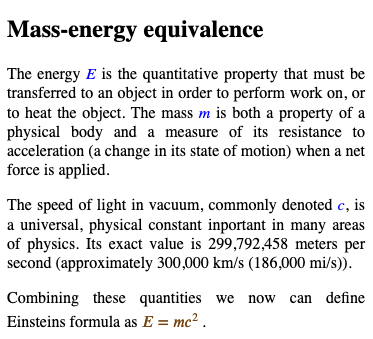
\includegraphics[scale=0.25]{images/doc}
        \end{columns}
    \end{frame}

    \begin{frame}{What is a REPL?}
        \begin{columns}
        \column{0.5\textwidth}
            \begin{itemize}
                \item REPL = \textbf{R}ead \textbf{E}val \textbf{P}rint \textbf{L}oop
                \begin{enumerate}
                    \item\label{replbegin} Read a Command from the user
                    \item Evaluate the Command
                    \item Print the Result
                    \item Loop back to \ref{replbegin}
                \end{enumerate}
                \item commonly used for programming or command line interaction
                \begin{itemize}
                    \item e.g. Bash (Linux / Mac OS) or PowerShell (Windows)
                    \item e.g. Python (scientific programming)
                \end{itemize}
            \end{itemize}
        \column{0.5\textwidth}
            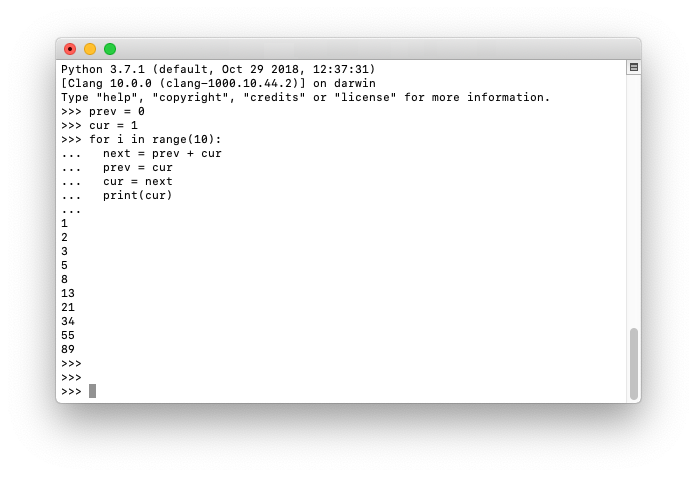
\includegraphics[scale=0.25]{images/repl}
        \end{columns}
    \end{frame}

    \begin{frame}{Notebooks + Jupyter}
        \begin{columns}
        \column{0.4\textwidth}
            \begin{itemize}
                \item Notebooks build on the REPL paradigm
                \item consist of a set of cells, each either have some code or documentation
                \item an OpenSource implementation \textbf{Jupyter} System
                \begin{itemize}
                    \item supports different programming languages using \textbf{kernels}
                \end{itemize}
                \item Interactive, but \textbf{requires programming}
            \end{itemize}
        \column{0.6\textwidth}
            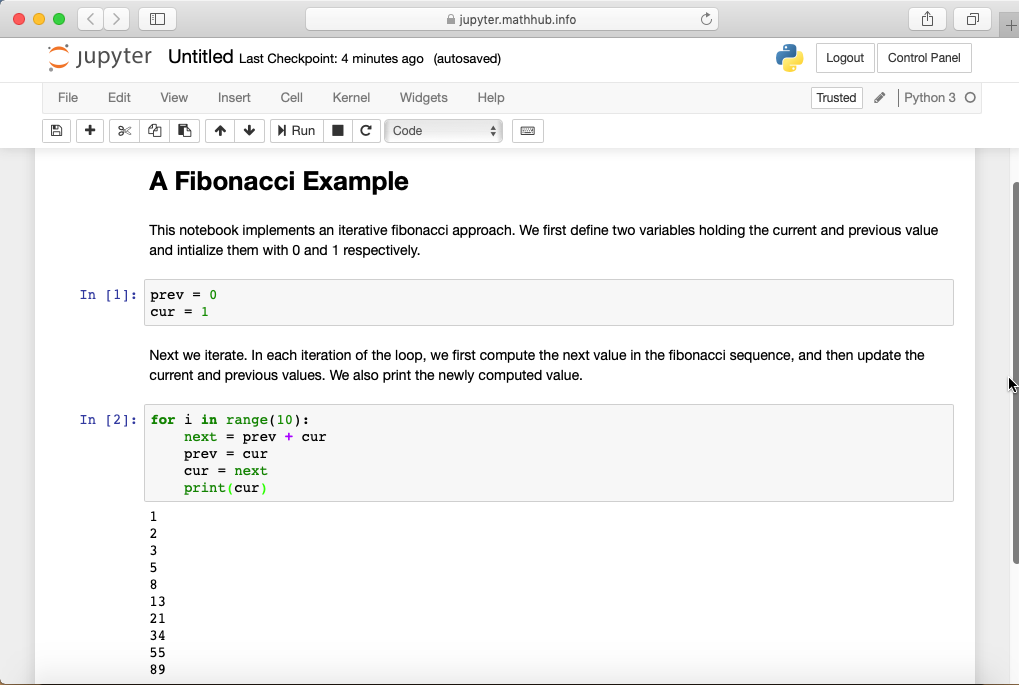
\includegraphics[scale=0.2]{images/notebook}
        \end{columns}
    \end{frame}

    \begin{frame}{OMDOC and MMT and MathHub}
        \begin{itemize}
            \item \textbf{OMDoc} = format for \textbf{O}pen \textbf{M}athematical \textbf{Doc}uments
            \begin{itemize}
                \item format for encoding STEM documents and knowledge
                \item developed mainly by \textit{Michael Kohlhase}
                \item can handle formal, informal and flexiformal content
                \begin{itemize}
                    \item formal = e.g. formalized proof, well-typed program, formal library
                    \item informal = e.g. paper, textbook, presentation
                    \item flexiformal = anything in-between, e.g. informal document with well-annotated formulae in between
                \end{itemize}
            \end{itemize}
        \end{itemize}
    \end{frame}

    \begin{frame}[fragile]{MMT}
        \begin{itemize}
            \item \textbf{MMT} = Meta-Meta-Tool
            \begin{itemize}
                \item framework for knowledge representation, implemented in Scala
                \item developed mainly by \textit{Florian Rabe}
                \item avoids a specific representational paradigm and is language-independent
                \item makes use of OMDOC, can thus handle formal, informal and flexi-formal documents
            \end{itemize}
            \item Knowledge is modeled using theory graphs
            \begin{itemize}
                \item theory = collection of declarations 
                \item declaration = represents a \textbf{symbol}, \textbf{statement} or \textbf{property}
                \item theory graphs = theories and relations between them, e.g. truth-preserving mappings or extensions
            \end{itemize}
        \end{itemize}
        \begin{figure}[!h]
\centering
\def\cn#1{\ensuremath{\mathsf{#1}}}
\def\gray#1{\textcolor{gray}{#1}}
\begin{tikzpicture}[xscale=.7,yscale=.8]\footnotesize
  \node[thy] (Mon) at (0,1.2)
  {$\mmtthy{Monoid}{\gray{\cn{U},\;\cn{op},\;\cn{e},\; \cn{unit}}}{}$};
  \node[thy] (CGr) at (0,3) {$\mmtthy{CGrp}{\gray{\cn{i},\;\cn{inv},\;\cn{comm}}}{}$};
  \node[thy] (Ring) at (-3.5,3) {$\mmtthy{Ring}{\gray{\cn{dist}}}{}$};
  \draw[include](Mon) -- (CGr);
  \draw[struct](CGr) -- node[below]{$\cn{add}$}(Ring);
  \draw[struct](Mon) -- node[left]{$\cn{mul}$} (Ring);
\end{tikzpicture}
\end{figure}
    \end{frame}

    \begin{frame}{MathHub}
        \begin{columns}
        \column{0.4\textwidth}
            \begin{itemize}
                \item \textbf{MathHub} \url{https://mathhub.info/}
                \begin{itemize}
                    \item portal for active mathematical documents and an archive for flexiformal mathematics
                    \item uses MMT as a backend and OMDoc as a representational format
                \end{itemize}
            \end{itemize}
        \column{0.6\textwidth}
            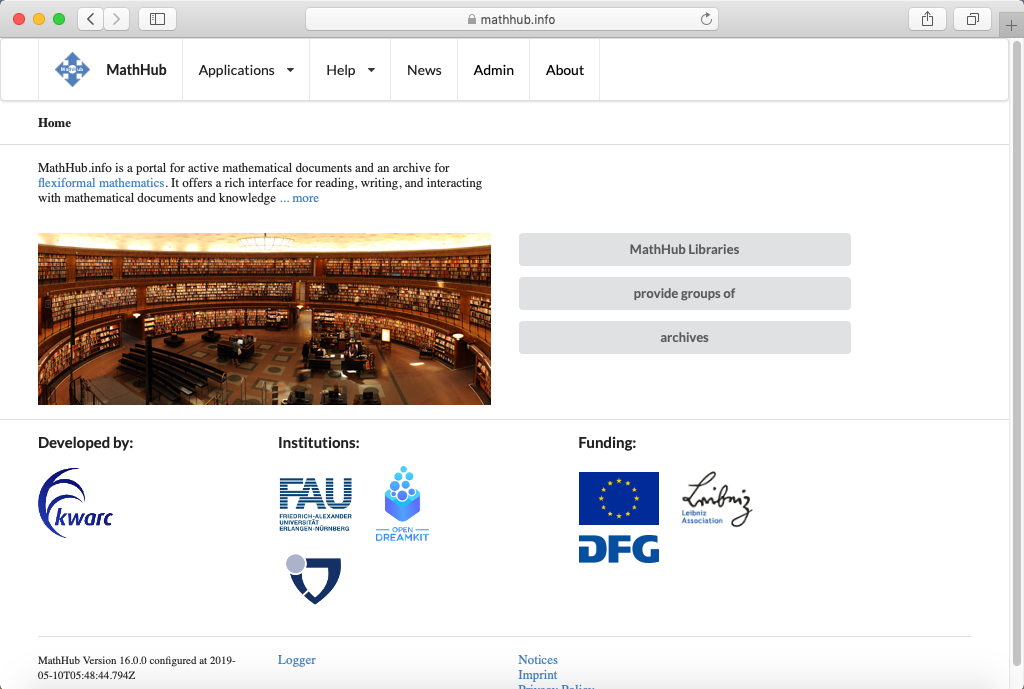
\includegraphics[scale=0.2]{images/mathhub}
        \end{columns}
    \end{frame}

    \begin{frame}{Goals and Challenges}
        \begin{itemize}
            \item \textbf{Idea:} Combine interactive notebooks and static, semantically-annotated documents to get interactivity with little programming
            \begin{itemize}
                \item How can we combine the notebook and document paradigms?
                \item How can we support flexible interactions without forcing authors to pro-
gram?
            \end{itemize}

            \item Our solution
            \begin{itemize}
                \item Make use of \textbf{OMDOC} as it can represent flexi-formal documents
                \item Import them into MMT
                \item Build a \textbf{Jupyter Kernel} for an MMT REPL
                \item Expand this Kernel to support Widgets \textit{(more on what exactly those are later)}
                \item Make the result accessible directly from within documents
            \end{itemize}

            \item This talk: Key design choices + overview of the implementation + some examples
            \begin{itemize}
                \item \textit{Read the paper for more details}
            \end{itemize}
        \end{itemize}
    \end{frame}

    \begin{frame}{Overview}

        \begin{itemize}
            \item This talk: Key design choices + overview of the implementation + some examples
            \begin{itemize}
                \item \textit{Read the paper for more details}
            \end{itemize}
        \end{itemize}

        \begin{enumerate}
            \item Introduction
            \item A REPL for MMT
            \item Widgets for active documents
            \item Conclusion
        \end{enumerate}
    \end{frame}

    \section{A REPL for MMT}

    \begin{frame}{Architecture of Jupyter and Kernels}
        \begin{itemize}
            \item Frontend: Implemented using \textbf{TypeScript} in the browser
            \item Backend: Implemented using \textbf{Python}
            \begin{itemize}
                \item programming-language features delegated to \textbf{language-specific} kernels
            \end{itemize}
            \item Kernels communicate with the backend using a dedicated protocol
            \begin{itemize}
                \item provide a REPL-style interface
                \item also support widgets \textit{(more on this later)}
                \item can in principle be implemented in any language
                \item usually written in the language they offer support for
            \end{itemize}
            \item We want to build a Jupyter kernel + REPL for MMT
        \end{itemize}
    \end{frame}

    \begin{frame}{A Jupyter Kernel for MMT}
        \begin{itemize}
            \item Opening a notebook = starting a \textbf{new session}
            \begin{itemize}
                \item each session contains a set of commands
                \item similar to an MMT document = set of declarations
                \item declaration = \textbf{symbol} and optional \textbf{definition} and \textbf{type}
            \end{itemize}
            \item principle: create a new MMT document for each session
            \begin{itemize}
                \item each input generates a new declaration within the current document
                \item definition is the input of the user
            \end{itemize}
            \item Recall: MMT is language and semantics independent
            \begin{itemize}
                \item definitions may contained \textbf{unevaluated} symbols
                \item they may not be simplified
            \end{itemize}
            \item MMT also supports nesting of documents
            \item $\Rightarrow$ it is not sufficient to provide only commands to write declarations
        \end{itemize}
    \end{frame}

     \begin{frame}{Messages in the Jupyter Kernel}
        \begin{itemize}
            \item Opening a notebook = starting a \textbf{new session}
            \begin{itemize}
                \item each session contains a set of commands
                \item similar to an MMT document = set of declarations
                \item declaration = \textbf{symbol} and optional \textbf{definition} and \textbf{type}
            \end{itemize}
            \item principle: create a new MMT document for each session
            \begin{itemize}
                \item each input generates a new declaration within the current document
                \item definition is the input of the user
            \end{itemize}
            \item Recall: MMT is language and semantics independent
            \begin{itemize}
                \item definitions may contained \textbf{unevaluated} symbols
                \item they may not be simplified
            \end{itemize}
            \item MMT also supports nesting of documents
            \item $\Rightarrow$ it is not sufficient to provide only commands to write declarations
        \end{itemize}
    \end{frame}

    \begin{frame}{Commmands in the MMT Kernel}
        \begin{itemize}
            \item Global Management commands
            \begin{itemize}
                \item manage sessions, e.g. display, create and delete all sessions
                \item should not be exposed to the average user
            \end{itemize}
            \item Local management commands
            \begin{itemize}
                \item start, quit, restart the current session
                \item change the context of the current session
                \item usually issued automatically by the kernel
            \end{itemize}
           \item Content Commands
            \begin{itemize}
                \item Write-Commands: Add new content to the MMT backend
                \item Read-Commands: Retrieve existing content or transform it (e.g. simplification)
                \item Interactive-Commands: Used for widgets \textit{(later)}
            \end{itemize}
            \item Recall: MMT is language and semantics independent
            \begin{itemize}
                \item definitions may contained \textbf{unevaluated} symbols
                \item they may not be simplified
            \end{itemize}
        \end{itemize}
    \end{frame}

    \begin{frame}{A sample notebook}
         \begin{columns}
        \column{0.5\textwidth}
            \centering
            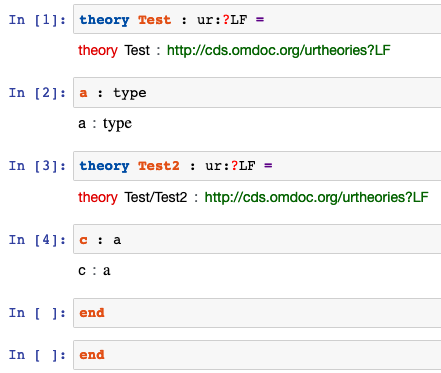
\includegraphics[scale=0.4]{images/notebooknested}
        \column{0.5\textwidth}
            \centering
            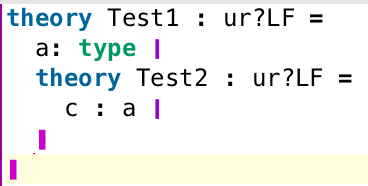
\includegraphics[scale=0.8]{images/theorynested}
        \end{columns}
    \end{frame}


    \begin{frame}{MMT Kernel Architecture}
        \begin{columns}
        \column{0.5\textwidth}
            \begin{itemize}
                \item Implementation consists of three layers
                \begin{enumerate}
                    \item Top Layer: Jupyter Kernel written in Python
                    \item Middle Layer: MMT Kernel written in Scala
                    \item Bottom Layer: MMT REPL written in Scala
                \end{enumerate}
                \item The Top Layer communicates with the frontend via Jupyter
                \item The Top and Middle layer communicate via a Python-JVM bridge called \textbf{Py4J}
            \end{itemize}
            \column{0.5\textwidth}
            \centering
            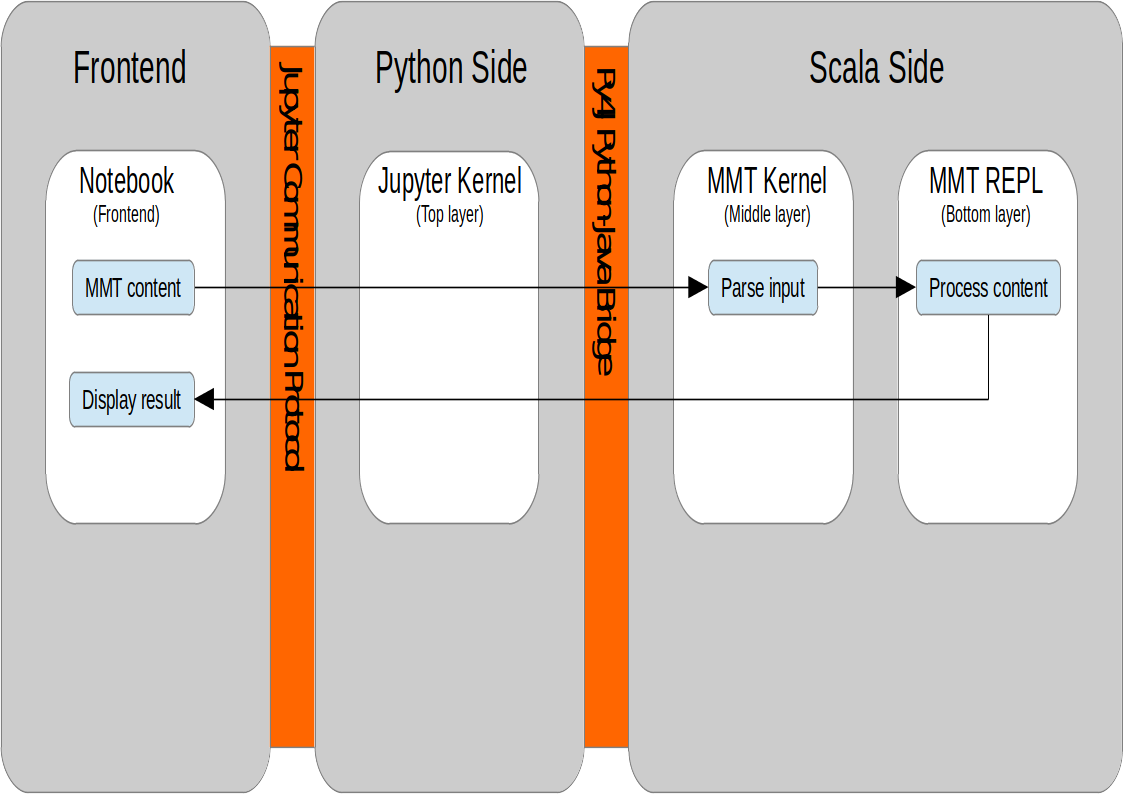
\includegraphics[scale=0.2]{images/eval}
        \end{columns}
    \end{frame}

    \section{Widgets for Active Documents}

    \begin{frame}{An Introduction to Widgets}
        \begin{itemize}
            \item widgets = \textbf{GUI component} that allows Jupyter kernels to provide graphical interfaces
            \begin{itemize}
                \item e.g. button, slider, input field, output field, labels, ...
                \item go \textbf{beyond} the REPL paradigm
            \end{itemize}

            \item can be plugged together interactively
            \item consist of kernel-side and frontend code
            \begin{itemize}
                \item frontend contains HTML, CSS + JavaScript
                \item kernel holds the state of the widget
            \end{itemize}
            \item Kernels can implement custom widgets by plugging together existing ones
        \end{itemize}
    \end{frame}

    \begin{frame}{An example: The active computation widget}
        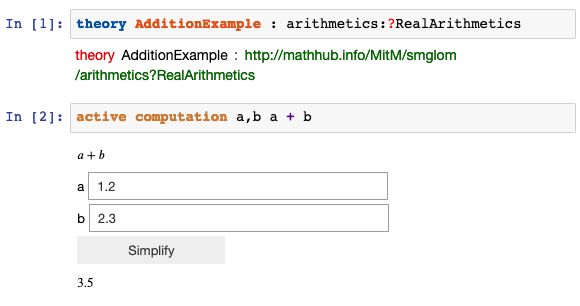
\includegraphics[scale=.5]{images/activecomp}
        \begin{itemize}
            \item the user can enter a \textbf{term} and a \textbf{set of variables}
            \item widget allows to change the variables and compute the result
        \end{itemize}
    \end{frame}

    \begin{frame}{MMT Kernel Widget Architecture}
        \centering
        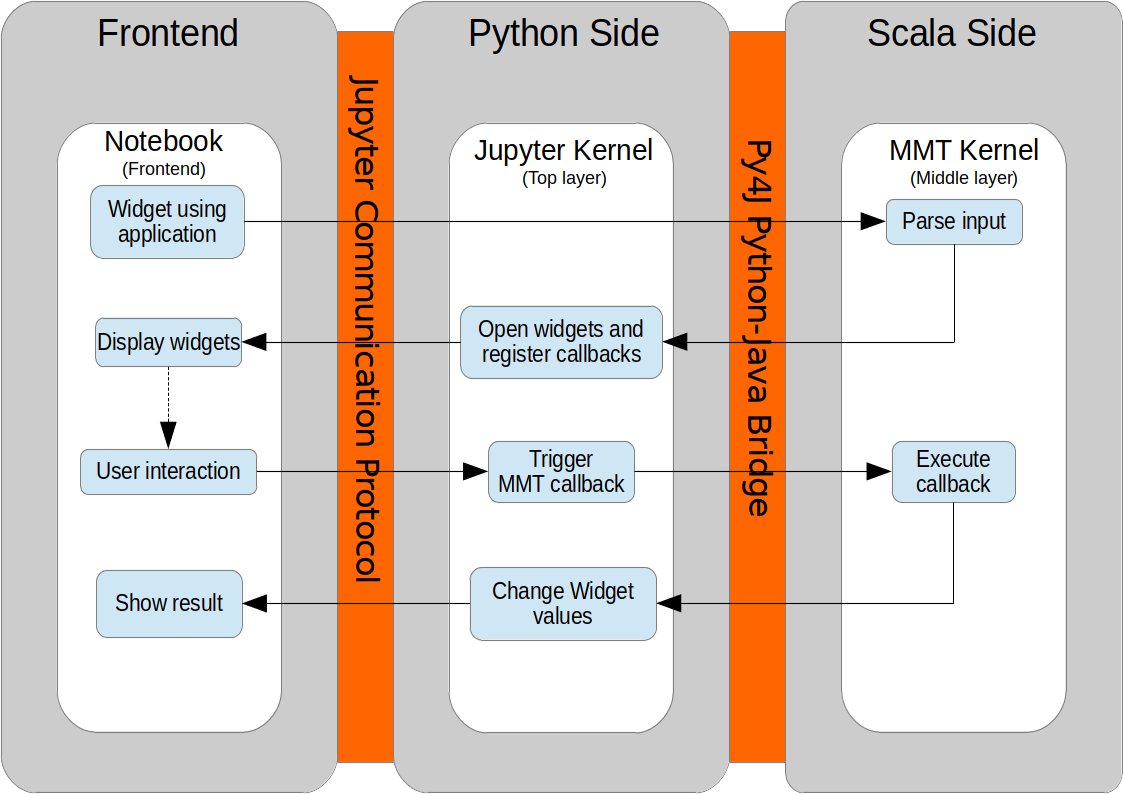
\includegraphics[scale=.35]{images/widgets}
    \end{frame}

    \begin{frame}[fragile]{Widgets inside Static Documents}
        \begin{itemize}
            \item \textbf{Idea: } Make this usable directly from documents
            \begin{itemize}
                \item We need to know \textbf{the formula} that we want to interact with
                \begin{itemize}
                    \item Let the user click on it
                \end{itemize}
                \item We need to know the \textbf{context} and \textbf{variables}
                \begin{itemize}
                    \item Annotate them on the document
                \end{itemize}
            \end{itemize}
        \end{itemize}

        \begin{columns}
        \column{0.35\textwidth}
            \centering
            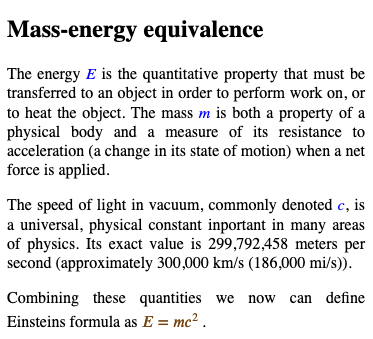
\includegraphics[scale=0.25]{images/doc}
        \column{0.65\textwidth}
            \lstset{
  basicstyle=\scriptsize\sffamily,
  columns=fullflexible,
  showstringspaces=false,
  commentstyle=\color{gray}\upshape,
  morestring=[b]",
  morestring=[s]{>}{<},
  morecomment=[s]{<?}{?>},
  stringstyle=\color{black},
  identifierstyle=\color{blue},
  keywordstyle=\color{cyan},
}
\begin{lstlisting}
<h2>Mass-energy equivalence</h2>
<div data-theory="?MEC">
 <p>The energy
  <math data-declares="E"><mi>E</mi></math>
  ... The speed of light in vacuum ... 
  <math data-declares="c"><mi>c</mi></math> ...
 </p>
 <p>We can now define Einsteins formula as 
  <math data-declares="m,c">E=mc^2</math>.</p>
</div>
\end{lstlisting}

        \end{columns}
    \end{frame}

    \begin{frame}[fragile]{Widgets inside Static Documents (2)}
        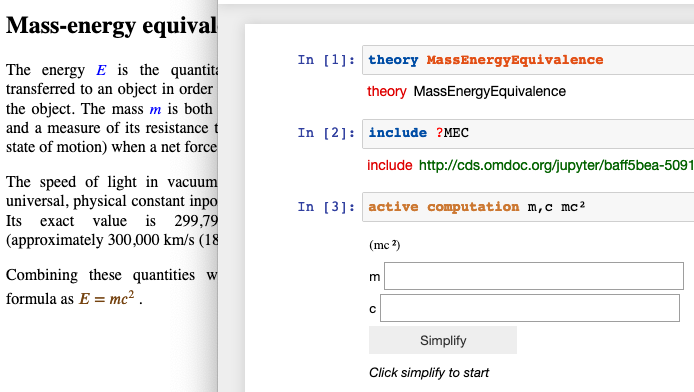
\includegraphics[scale=0.5]{images/acwidget}
    \end{frame}


    \section{Conclusion}

    \begin{frame}{Conclusion}
        \begin{itemize}
            \item We have presented an integration of Documents and Notebooks
            \begin{itemize}
                \item based on \textbf{OMDoc} and \textbf{MMT}
                \item consists of a \textbf{Jupyter Kernel} with widget support
                \item initial integration into \textbf{Active Documents}
            \end{itemize}

            \item We have only given an overview here, and shown a few examples
            \begin{itemize}
                \item Read the paper for more details!
            \end{itemize}

            \item Still a lot of work left!
            \begin{itemize}
                \item Deep MathHub/Jupyter Integration
                \item IDE Support for Documents with Active Computation
                \item REPL Cells/Documents as first-class citizens in MMT
                \item and more $\dots$
            \end{itemize}

            \item Questions, Comments, Concerns?

            \item Thank You For Listening!

        \end{itemize}
    \end{frame}

\end{document}